% Objet : fleche avec un texte au milieu 
% Paramètres : point de départ, taille, texte

\newcommand{\fleche}[3]{
	\draw[<-, >=stealth, thick] (#1) -- +(#2);
	\path (#1) -- +(#2) node[midway, above] {#3};
}


% Objet : sous-blocs: x, y, largeur, hauteur, titre
\newcommand{\sousbloc}[5]{
	\begin{scope}[shift={(#1,#2)}]
		\draw[fill=gray!40] (0,0) rectangle (#3,#4);
		\node[anchor=north west] at (0.05,#4-0.1) {\small #5};
	\end{scope}
}

% Objet : blocs
\newcommand{\bloc}[3]{
	\begin{scope}[shift={(#1,#2)}]
		\draw[rounded corners=0.2cm, fill=gray!20] (0,0) rectangle (6,4.7);
		
		% Titre en haut à gauche
		\node[anchor=north west] at (0.2,4.5) {\textbf{#3}};

		% Premiere ligne : hash du bloc précédent + nonce
		\sousbloc{0.3}{3}{3.4}{0.7}{Hash du préc. bloc}
		\sousbloc{4}{3}{1.7}{0.7}{Nonce}
		
		% Deuxième ligne : reste du header
		\sousbloc{0.3}{2}{5.4}{0.7}{Reste du header}

		% Troisième ligne : données applicatives
		\sousbloc{0.3}{0.3}{5.4}{1.4}{Données applicatives}

	\end{scope}
}


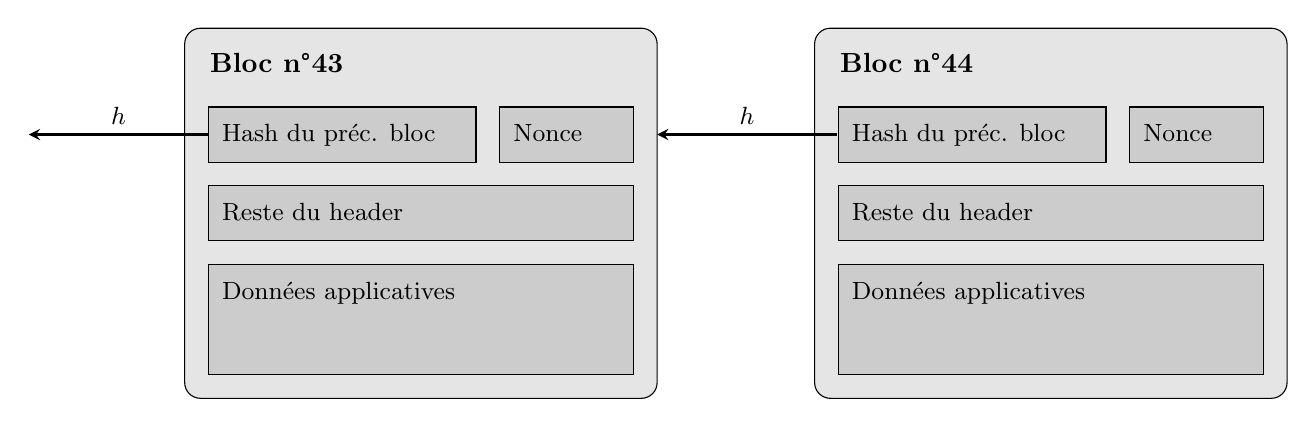
\begin{tikzpicture}[scale=1]
	\begin{scope}[shift={(3cm,-5cm)}, fill opacity=1]
		\bloc{0}{0}{Bloc n°43}
		\bloc{8}{0}{Bloc n°44}

		\fleche{6,3.35}{2.28, 0}{\small $\mathfrak{h}$}
		\fleche{-1.98,3.35}{2.28,0}{\small $\mathfrak{h}$}


		% Add more blocs as needed
	\end{scope}
\end{tikzpicture}